%%%%%%%%%%%%%%%%%%%%%%%%%%%%%%%%%%%%%%%%%%%%%%%%%%%%%%%%%%%%%%%%%%%%%%%%%%%%%%%%
%2345678901234567890123456789012345678901234567890123456789012345678901234567890
%        1         2         3         4         5         6         7         8

\documentclass[letterpaper, 10 pt, conference]{ieeeconf}  % Comment this line out if you need a4paper

%\documentclass[a4paper, 10pt, conference]{ieeeconf}      % Use this line for a4 paper

\IEEEoverridecommandlockouts                              % This command is only needed if 
                                                          % you want to use the \thanks command

\overrideIEEEmargins                                      % Needed to meet printer requirements.

%In case you encounter the following error:
%Error 1010 The PDF file may be corrupt (unable to open PDF file) OR
%Error 1000 An error occurred while parsing a contents stream. Unable to analyze the PDF file.
%This is a known problem with pdfLaTeX conversion filter. The file cannot be opened with acrobat reader
%Please use one of the alternatives below to circumvent this error by uncommenting one or the other
%\pdfobjcompresslevel=0
%\pdfminorversion=4

% See the \addtolength command later in the file to balance the column lengths
% on the last page of the document

% The following packages can be found on http:\\www.ctan.org
\usepackage{graphics} % for pdf, bitmapped graphics files
\usepackage{epsfig} % for postscript graphics files
\usepackage{mathptmx} % assumes new font selection scheme installed
\usepackage{times} % assumes new font selection scheme installed
\usepackage{amsmath} % assumes amsmath package installed
\usepackage{amssymb}  % assumes amsmath package installed
\usepackage{listings}
\usepackage[latin1]{inputenc}
\usepackage{epigraph}
\usepackage{cleveref}
\usepackage{booktabs}
\usepackage{url}
\usepackage{xcolor}
\usepackage{tabularx}
\usepackage{siunitx}
\usepackage[nolist]{acronym}
\graphicspath{{images/}}
\usepackage{float}
\usepackage{framed}
\hyphenchar\font=-1


%%%%%%%%%%%%%%%%%%%%%%%%%%%%%%%%%%%%%%%%%%%%%%%%%%%%%%%%%%%%%%%%%%%%%%
%%																	%%
%%						Title and Author							%%
%%																	%%
%%%%%%%%%%%%%%%%%%%%%%%%%%%%%%%%%%%%%%%%%%%%%%%%%%%%%%%%%%%%%%%%%%%%%%
\title{\LARGE \bf
	Development of an autonomous driving environment model visualization based on object list level
}

\author{Christoph Zach, Denis R�sler, Dominik Knauer, Maximilian Pfaller,\\ Maximilian Haindl, Philipp Korn, Stephan Schweigard and Tobias Wagner
%	\thanks{*This work was not supported by any organization}% <-this % stops a space
}


%%%%%%%%%%%%%%%%%%%%%%%%%%%%%%%%%%%%%%%%%%%%%%%%%%%%%%%%%%%%%%%%%%%%%%
%%																	%%
%%							Document								%%
%%																	%%
%%%%%%%%%%%%%%%%%%%%%%%%%%%%%%%%%%%%%%%%%%%%%%%%%%%%%%%%%%%%%%%%%%%%%%
\begin{document}
	\maketitle
	\thispagestyle{empty}
	\pagestyle{empty}
	\begin{acronym}[slmtA]
		\acro{GT}{Ground-Truth}
		\acro{YOLO}{You Only Look Once}
		\acro{ROS}{Robot Operating System}
		\acro{API}{application programming interface}
		\acro{ID}{identifier}
		\acro{TP}{True Positive}
		\acro{FP}{False Positive}
		\acro{FN}{False Negative}
		\acro{mm}{mismatch}
		\acro{IoU}{Intersection over Union}
		\acro{RVIZ}{3D visualization tool}
		\acro{GUI}{Graphical User Interface}
	\end{acronym}
	%%%%%%%%%%%%%%%%%%%%%%%%%%%%%%%%%%%%%%%%%%%%%%%%%%%%%%%%%%%%%%%%%%%%%%%%%%%%%%%%%%
	%%									Abstract									%%
	%%%%%%%%%%%%%%%%%%%%%%%%%%%%%%%%%%%%%%%%%%%%%%%%%%%%%%%%%%%%%%%%%%%%%%%%%%%%%%%%%%

%	\begin{abstract}
		\begin{abstract}

Simulating vehicle test scenarios, detecting objects with a camera sensor and analyzing the resulting object detections afterwards - in this paper it is described how this can be performed using several applications. Within the scope of a students' project the development environment is created and the quality of object detections by a simulated camera sensor is evaluated with a generated post-processing application.

\end{abstract}
		
	
	%%%%%%%%%%%%%%%%%%%%%%%%%%%%%%%%%%%%%%%%%%%%%%%%%%%%%%%%%%%%%%%%%%%%%%%%%%%%%%%%%%
	%%									Introduction								%%
	%%%%%%%%%%%%%%%%%%%%%%%%%%%%%%%%%%%%%%%%%%%%%%%%%%%%%%%%%%%%%%%%%%%%%%%%%%%%%%%%%%
%	\begin{figure*}[!h]
%		\centering
%		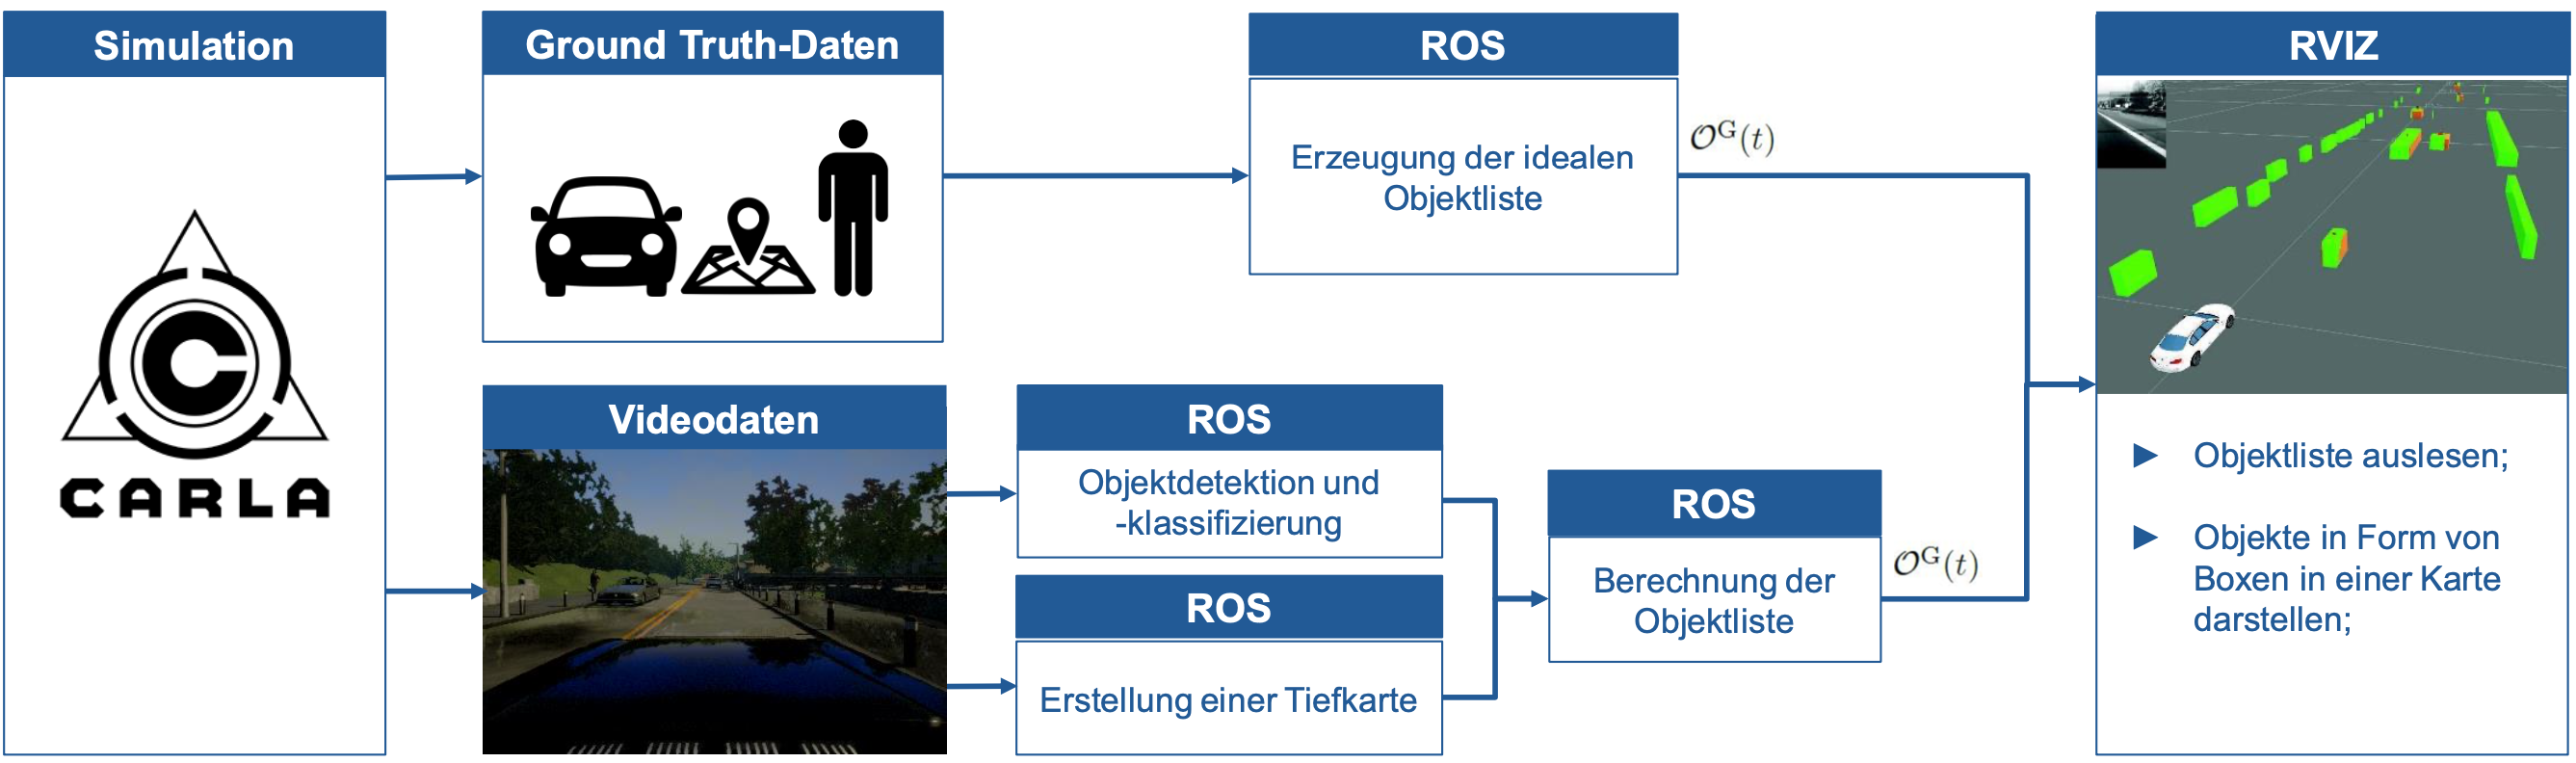
\includegraphics[width=0.85\linewidth]{images/Ueberblick}
%		\caption{Overview}
%		\label{fig:Overview}
%	\end{figure*}
	\section{INTRODUCTION}
	Camera data and its camera-based algorithms are increasingly being used to make people, vehicles, objects and buildings visible for automated vehicles. With the help of these algorithms, the raw camera data can be evaluated regarding to various criteria. Important distinctions are the classification, dimensions, distance, alignment and the relative speed of the detected objects in relation to the ego-vehicle \cite{Aeberhard}. \ac{YOLO} is one of the most effective real-time object detection algorithms and offers all of these functions \cite{knuthwebsite}.
Due to the fact that new driving functions usually be validated on a proving ground under controlled conditions, environment simulation software such as CARLA are used instead for developing, training and validating driving systems\cite{Gap}. CARLA is an open-source urban driving simulator for autonomous driving research which supports flexible sensor suits, user scripts and full control of all static and dynamic actors and maps \cite{Dosovitskiy17}. This offers the possibility to validate the camera data sets using different kind of camera-based algorithms for object detection or in addition to train them. To evaluate the Ground-Truth Data with the calculated algorithm objects, \ac{ROS} offers the possibility of sending the respective data streams using objects lists and evaluating them with a \ac{RVIZ} \cite{ROS}.
In this work, an autonomous driving environment model visualization based on an object list level is presented by using a NCAP test scenario for testing automated driving systems. An analysis is made based on the \ac{YOLO} camera object detection algorithm compared to the Ground-Truth Data directly generated from the environment simulation software model. \Cref{fig:Overview} illustrates the basic process flows for generating all data, visualizing and validating the results.


%Camera data and its camera-based algorithms are increasingly being used to make people, vehicles, objects and buildings visible for automated vehicles. With the help of these algorithms, the raw camera data can be evaluated regarding to various criteria. Important distinctions are the classification, dimensions, distance, alignment and the relative speed of the detected objects in relation to the ego-vehicle \cite{Aeberhard}. \ac{YOLO} is one of the most effective real-time object detection algorithms and offers all of these functions \cite{knuthwebsite}.
%Due to the fact that new driving functions usually be validated on a proving ground under controlled conditions, environment simulation software such as CARLA can be used instead for developing, training and validating driving systems\cite{Gap}. CARLA is an open-source urban driving simulator for autonomous driving research and supports flexible sensor suits, user scripts and full control of all static and dynamic actors and maps \cite{Dosovitskiy17}. This offers the possibility to validate the camera data sets using different kind of camera-based algorithms for object detection or in addition to train them. To evaluate the Ground-Truth Data with the calculated algorithm objects, \ac{ROS} offers the possibility of sending the respective data streams using objects lists and evaluating them with a \ac{RVIZ} \cite{ROS}.
%In this work, an autonomous driving environment model visualization based on an object list level is presented by using a NCAP test scenario for testing automated driving systems. An analysis is made based on the \ac{YOLO} camera object detection algorithm compared to the Ground-Truth Data directly generated from the environment simulation software model. \Cref{fig:Overview} illustrates the basic process flows for generating all data, visualizing and validating the results.




%Camera data and its camera-based algorithms are increasingly being used to make people, vehicles, objects and buildings visible for automated vehicles. With the help of these algorithms, the raw camera data can be evaluated regarding to various criteria. Important distinctions are the classification, dimensions, distance, alignment and the relative speed of the detected objects in relation to the ego-vehicle \cite{Aeberhard}. \ac{YOLO} is one of the most effective real-time object detection algorithms and offers all of these functions \cite{knuthwebsite}.
%Due to the fact that new driving functions usually be validated on a proven ground under controlled conditions, environment simulation software such as CARLA is used in the early development processes \cite{Gap}. 
%
%%\begin{center}
%%	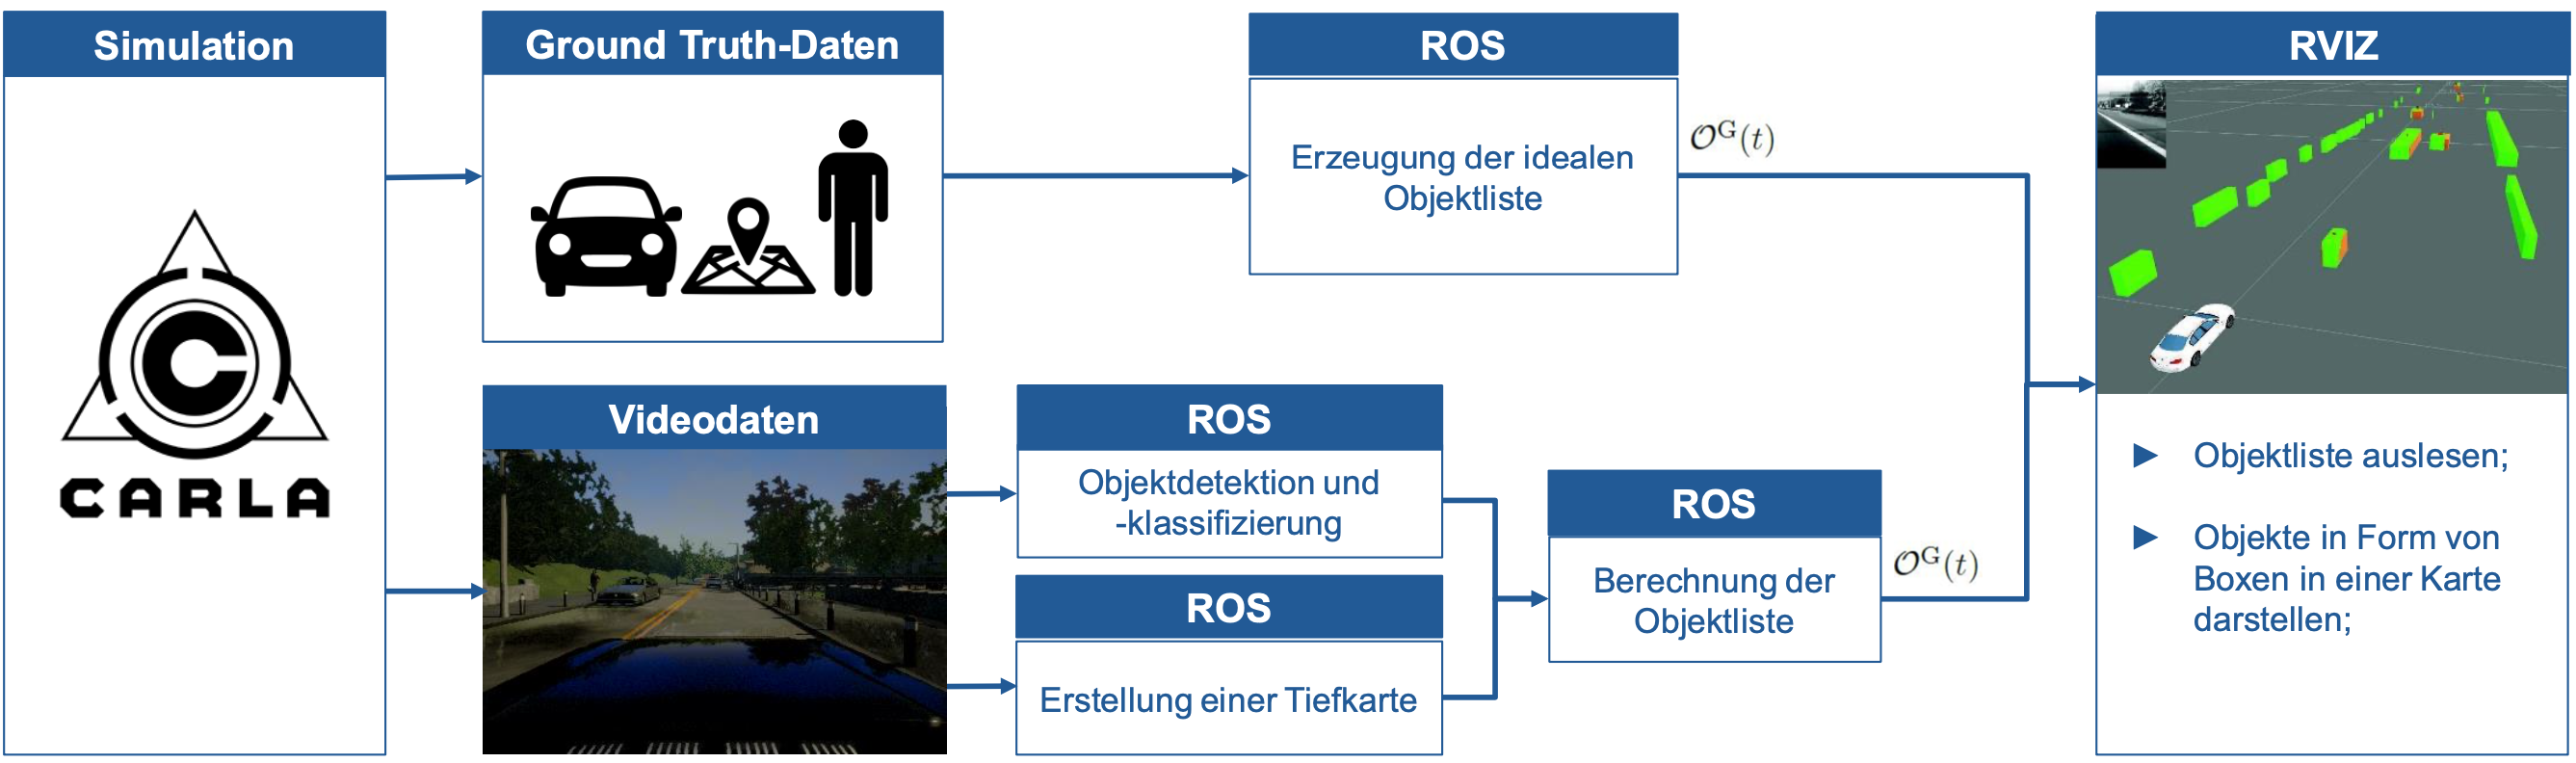
\includegraphics[width=2\linewidth]{images/Ueberblick}
%%	\captionof{figure}{My caption}
%%	\label{fig:mc-1}
%%\end{center}\newpage
%
%CARLA is an open-source urban driving simulator for autonomous driving research and supports flexible sensor suit and full control of all static and dynamic actors and maps \cite{Dosovitskiy17}. This offers the possibility to validate the camera data sets using different kind of camera-based algorithms for object detection or to train them quickly and easily. To evaluate the Ground-Truth Data of the simulation with the calculated algorithm objects, \ac{ROS} offers the possibility of sending the respective data streams using objects lists and evaluating them with a \ac{RVIZ} \cite{ROS}.
%In this work, an autonomous driving environment model visualization based on an object list level is presented by using a NCAP test scenario for testing automated driving systems. An analysis is made based on the \ac{YOLO} camera object detection algorithm compared to the Ground-Truth Data directly generated out of the environment simulation software model. !!!!HIER WUERDE ICH DIE OVERVIEW GRAFIK ERWAEHNEN UND DIREKT DARUNTER AM ENDE DER SEITE POSITIONIEREN, KANN ABER SCHWIERIG WERDEN, DA NOCH ABSTRACT FEHLT!!! \Cref{fig:Overview}
%
%
%

	
	
	%%%%%%%%%%%%%%%%%%%%%%%%%%%%%%%%%%%%%%%%%%%%%%%%%%%%%%%%%%%%%%%%%%%%%%%%%%%%%%%%%%
	%%									Related Works								%%
	%%%%%%%%%%%%%%%%%%%%%%%%%%%%%%%%%%%%%%%%%%%%%%%%%%%%%%%%%%%%%%%%%%%%%%%%%%%%%%%%%%

	\section{RELATED WORKS}
	
For detecting objects in an environment an object description model is necessary. This work is based on the model introduced in \cite{Aeberhard} which depicts an object through vectors and values shown in \cref{fig:vectors}.
To compare objects lists with each other and to evaluate detected objects the authors of \cite{Reway} developed a test method. It presumes the existence of an objects list and the associated GT dataset, therefore this work concentrates on creating these lists. To investigate the quality of the created objects lists, metrics of \cite{Reway} are used.


	
	
	%%%%%%%%%%%%%%%%%%%%%%%%%%%%%%%%%%%%%%%%%%%%%%%%%%%%%%%%%%%%%%%%%%%%%%%%%%%%%%%%%%
	%%							Materials and Methods								%%
	%%%%%%%%%%%%%%%%%%%%%%%%%%%%%%%%%%%%%%%%%%%%%%%%%%%%%%%%%%%%%%%%%%%%%%%%%%%%%%%%%%
	\section{MATERIALS AND METHODS}
	
\subsection{Creating objects list of Ground-Truth Data}
The first subsection deals with the used Software to create the test environment and the test scenario itself. CARLA is an open-source urban driving simulator for autonomous driving research and supports flexible sensor suites and full control of all static and dynamic actors and maps \cite{Dosovitskiy17}. The flexible \ac{API} and the \ac{ROS} integration provides a lot of flexibility and the possibility to extract the Ground-Truth Data directly from the scenario. The work is based on the CARLA 0.9.8 release combined with \ac{ROS} and python3 packages and a python3.5 founded \ac{API}. The test case is derived from the at Euro NCAP used Car-to-Pedestrian Nearside Child 50\,\% (CPNC-50) test scenario from the Insurance Institute for Highway Safety (IIHS) test protocol \cite{NCAP, Protocoll}. %und 3!
%TABLE 1: Test conditions pedestrian autonomous emergency braking (P-AEB) [4]
%\begin{table}[]
%	\begin{tabular}{|l|l|}
%	\hline
%	\textbf{Parameter}      & \textbf{CPCN-50 Scenario Child} \\ \hline
%	Test vehicle speed      & 40 km/h                   \\ \hline
%	Pedestrian target speed & 5 km/h                    \\ \hline
%	Target direction        & Crossing from R-to-L      \\ \hline
%	Target path             & Perpendicular             \\ \hline
%	Pedestrian dummy size   & Child                     \\ \hline
%	Overlap                 & 50 %                      \\ \hline
%	\end{tabular}
%\end{table}


\begin{table}[h]
	\caption{Test conditions pedestrian autonomous emergency braking (P-AEB) \cite{Protocoll}}
	\label{Test conditions}
	\begin{center}
		\begin{tabular}{l l}
			\hline
			Parameter & CPCN-50 Scenario Child\\
			\hline
			Test vehicle speed & 40 km/h\\
			Pedestrian target speed & 5 km/h\\
			Target direction        & Crossing from R-to-L\\
			Target path             & Perpendicular\\
			Pedestrian dummy size   & Child\\
			Overlap                 & 50 \%\\
			\hline
			
			
		\end{tabular}
	\end{center}
\end{table}



The test procedure starts with launching the test scenario by first spawning the three vehicles and the pedestrian to their initial positions into the map. This state consists of an Audi TT (1) in front and an Audi e-tron (2) arranged behind it. The left edges of both cars are parked 0.2 m away from the right edge of the test lane. The longitudinal distance between the cars and between the front car and pedestrian is 1.0 m, each. At the beginning of the simulation, the child pedestrian is positioned 7.0 m laterally from the center of the ego-vehicle, which is centered in its lane 200 m behind the pedestrian and portrayed as an Audi e-tron.

\begin{figure}[htbp]
	\centering
	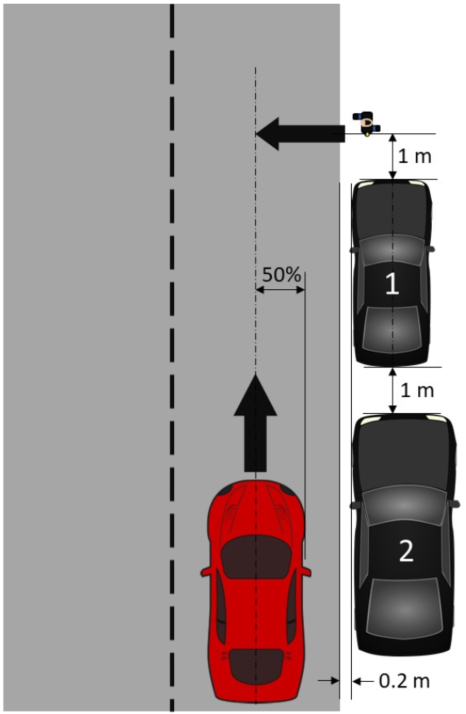
\includegraphics[width=0.23\textwidth]{images/Target_Placement_test_scenario.png}
	\caption{Target placement based on CPNC-50 test \cite{Protocoll}}
	\label{fig:coordination}
\end{figure}


After a few seconds, the ego vehicle starts accelerating quickly to 40 km/h and the child starts moving with constant speed from right-to-left to cross the street. The pedestrian becomes visible for the ego vehicle after he passed the Audi TT (2). The ego vehicle immediately engages an emergency brake and comes to a standstill in front of the child. At this point the pedestrian is at the 50\,\% overlapping point. The child continues crossing the street and the scenario ends as soon as the child completely passed the ego-vehicle.


\subsection{Creating objects list of Ground-Truth Data}
The Ground-Truth Data Objects List includes four message vectors for every spawned object\,-\,Classification, Dimension, Features and Geometric. These messages are used to classify the objects, send their geometrical dimensions, location, acceleration, angle and visible edges \cite{Aeberhard}.
The Classification parameters indicate the type of the spawned objects and differentiate between vehicle, pedestrian and other types. In addition, the Features vector contains all visible and invisible edges of the objects. The evaluation of both messages is statically generated for this scenario referring to the bounding box data of every spawned object. The third message represents the length, width and height of the object. This Dimensions vector receives the information as well from the bounding box. Furthermore, the Geometric message is used to represent the coordinates, speed, yaw angle and acceleration of the objects relative to the ego vehicle. 
The Ground-Truth Data will be published via \ac{ROS} in two different topics. Every topic includes a header with timestamp, object \ac{ID} as well as an Objects List message. This Objects List message includes all four messages for the pedestrian and both parked cars in topic one and is referenced to the center of the objects. Topic two includes only the Objects List message with the Geometric data of the ego vehicle based on the camera position at the front middle of the car.
The test scenario offers two options for publishing different data in topic one.
\begin{itemize}
	\item Publishing only Objects in the field of view of the camera (200 m and a total opening angle of \ang{60})
	\item Publishing all spawned objects over the whole test period
\end{itemize}

	\subsection{Creating object lists of camera data}\label{C}
\subsubsection{Object detection and preparation}
The first problem to deal with is to detect any possible object in every given frame. For that PyImageSearch published an useful version of a detection algorithm called \ac{YOLO} \cite{Yolo}. 
Changes in the code had to be made to use multiple frames instead of just one saved image stored on disk.
These frames of the simulation environment can be generated by in-game sensors like RGB and depth camera. It is necessary to place those cameras at the same spot on the ego-vehicle to collect comparable images without any errors by considering angular misalignment. As a result, the camera sensors will create images of 32-bit BGRA colors to work with. 
Because the \ac{YOLO} algorithm needs at least 0.35 seconds on every tested hardware the tick rate has to be synchronized and reduced to 0.5 seconds for both sensors.

To generate predominantly \ac{TP} cases, the confidence value of \ac{YOLO} is set to 0.7 and the threshold value to 0.6. Furthermore, tests in CARLA have resulted in \ac{FP} cases where objects such as umbrellas were detected. To exclude these cases, all irrelevant object classes are filtered out in advance. The bounding boxes are not used as usual to display them in the frame, but the pixel coordinates of the bounding boxes are used. These are composed of a \textit{x} and \textit{y} coordinate, as well as a width \textit{w} and height \textit{h} to determine the location of the detected object in the frame. In addition, the confidence and name of the detected objects are also used. 
\subsubsection{Data processing}
The resulting pixel coordinates of the bounding boxes can be used to cut out a frame of the specific object from the image. This is necessary to filter unsuitable pixel values and general noise in the image with an adaptive threshold filter. This filter also generates a black and white image that makes it possible to detect the silhouette of the given object. An evaluation of the blackened pixels and their resulting distances gives an approximate idea of the location in the simulation environment.
Therefore, the CARLA development team provides a formula (\cref{eq:distance}) to calculate the distance by using the color values of certain pixels of the depth image seen in \cref{fig:depth image} \cite{distance}. 

\begin{equation}
	\label{eq:distance}
	\begin{aligned}
		& (R, G, B) = v_{Pixel}\\
		& d_{norm} = (R+G*256+B*256*256)\,/\,(256*256*256-1)\\
		& d_{direct} = 1000 * d_{norm}\\
	\end{aligned}
\end{equation}
\begin{table}[!h]
	\begin{center}
		\begin{tabular}{l c l}
			$v_{Pixel}$ & = & color values of specific pixel\\
			$d_{norm}$ & = &  normalized displacement\\
			$d_{disp}$ & = & displacement of camera sensor and object\\
		\end{tabular}
	\end{center}
\end{table}


\begin{figure}[b]
	\centering
	\fbox{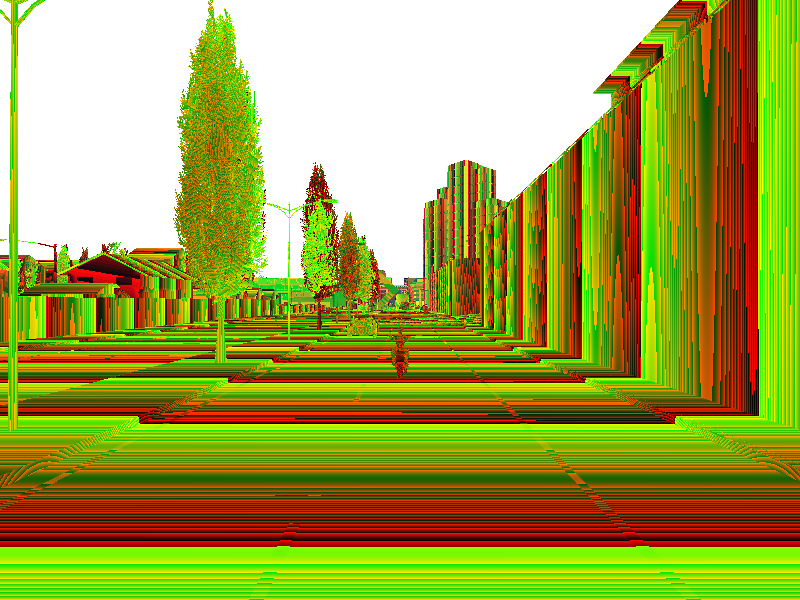
\includegraphics[width=0.4\textwidth]{depthimage.png}}
	\caption{Image codifying depth value via RGB color space}
	\label{fig:depth image}
\end{figure}

This makes it possible to determine not only the direct distance of any visible object, but also the length of the object itself. By processing the calculated distances in a frame it is possible to estimate the length. To get accurate results at this early stage the object has to be fully visible. Otherwise the length is an approximated estimation. 
This value is added to the previously calculated distance to obtain the center of an object. To get the final position in the simulation environment taking into account the rotation of an object, the yaw angle must be considered, too.\\

\subsubsection{Object Tracker}
Over time, new objects become visible and some disappear. For now, the detection algorithm cannot track them. In addition, depending on the movement, objects are not detected in the same order. To keep track of all objects it is necessary to identify already detected ones in the following frames. To do so, all bounding boxes must get connected with an unique \ac{ID}. For this purpose a function made available by PyImageSearch is used \cite{Tracker}. This tracker was chosen for the reason that it is just necessary to provide coordinates of the bounding boxes. The code recognizes the movement and links an ID to a specific object in the bounding box.\\
	\subsubsection{Generating an object list}
From the detected coordinates in form of x- and y-coordinates and a detected distance, the distance from the ego-vehicle, velocity, acceleration, angle of the object and angular velocity, can be calculated. For the calculation previous values are stored and assigned to an ID. With the proportionality of the object distance from the vertical centerline and the camera angle, the script scales in metric distance.

\begin{equation}
D_{Center} = Y_{Pixel} - \frac{FO_{Horizontal}}{2}
\label{test}
\end{equation}

This formula divides the image into two segments (left and right segment) and calculates the distance of the object to this center axis.

\begin{equation}
F  = \frac{D_{Center}}{L_{Pixel}}
\end{equation}

Here is a factor calculated, which corresponds to a value of -1...0 or 0...1. This indicates, which factor of the total segment width, the object is located.

\begin{equation}
\varphi = F * \measuredangle_{Camera}
\end{equation}

The angle of view from the camera, which corresponds to \ang{90}, is used. In relation to a segment, it would be \ang{45}. This is calculated with the factor, to get an angle related to the vertical axis.

\begin{figure}[h]
	\centering
	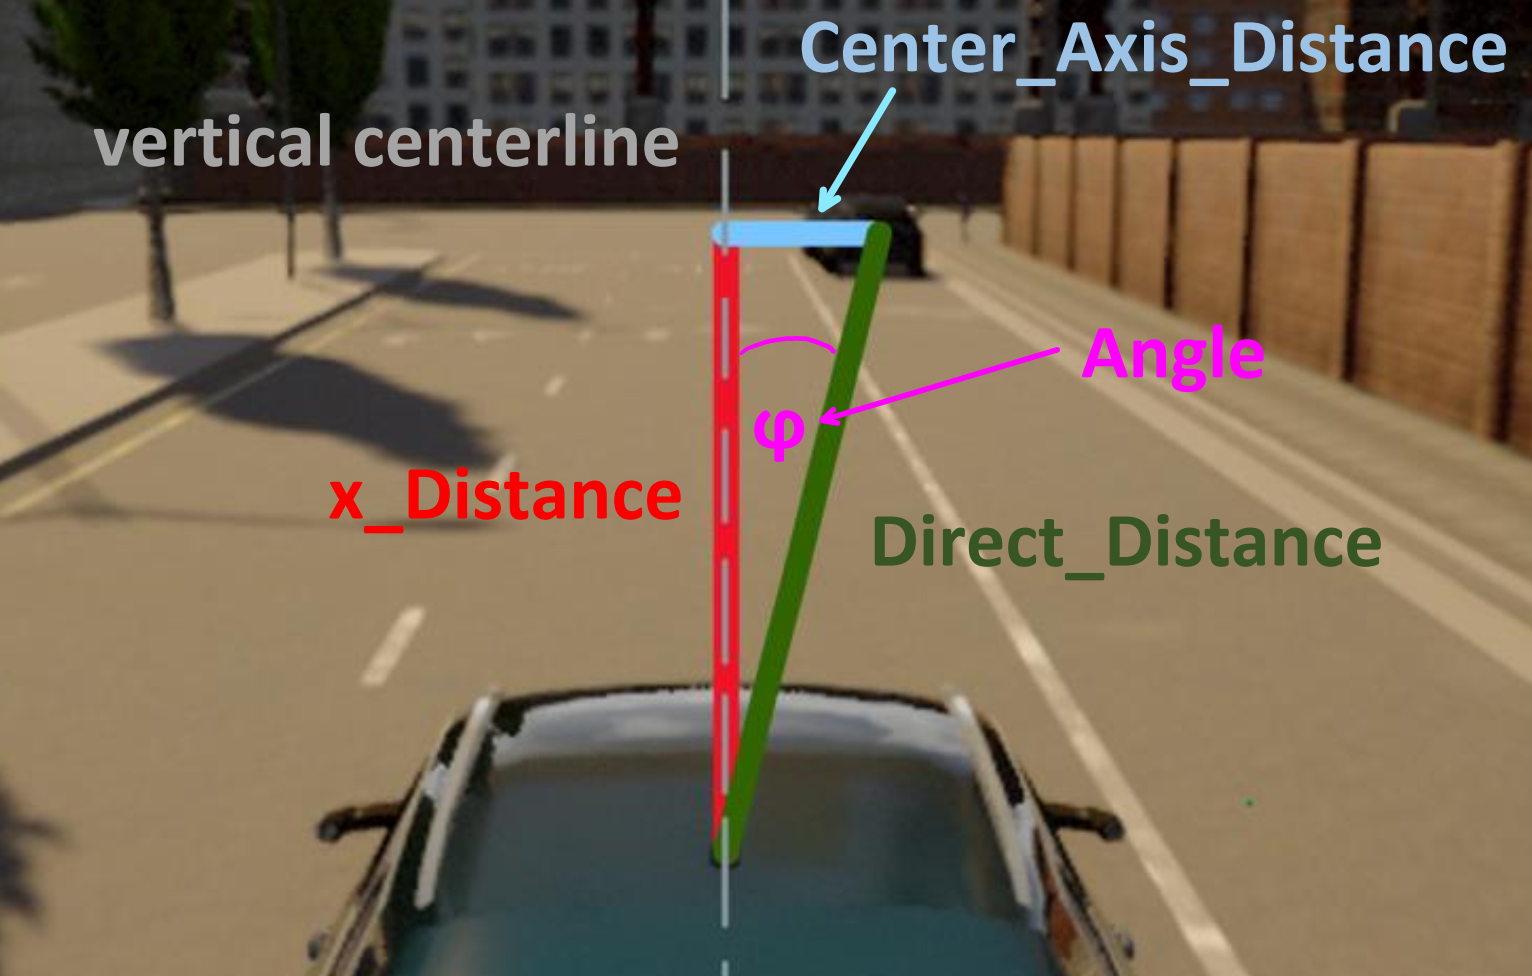
\includegraphics[width=0.4\textwidth]{images/calc_angle.png}
	\caption{Calculation of angle}
	\label{fig:anglecalculation}
\end{figure}

By using the angle and the direct distance, the trigonometric theorems can be used to calculate the x- and y-distance in meters, which are the basis for the velocity- , acceleration- , angle- , and angular velocity-calculation. The object attributes are stored over several frames to calculate time-dependent values. Velocity is calculated by the change of the x- and y-distances, the acceleration, by changing the x- and y-velocities. The angle with the Velocity in x- and y-direction and the angular velocity is calculated by time changing angles. The calculated values are related to the ego-vehicle.
The dimensioning is based on the same formulas. The formulas above are used to calculate an angle. This angle can be used, to calculate a distance in meters from the center vertical axis, for the position of the vehicle on the y-axis.

\begin{equation}
	Y_{Meter} = D_{Direct} * sin(\frac{\varphi * \pi}{180})
\end{equation}

After calculating the distance of the object to the center axis of the image, it is divided by the pixel distance of the object according to the center axis. This gives a meter per pixel value, to convert the detected object dimensions in pixels, to meter.

\begin{equation}
	D_{PerPixel} = \frac{Y_{Meter}}{D_{Center}}
\end{equation}

Via the \ac{ROS} Framework, the required data such as geometry, probability, \ac{ID} of the object etc. are transferred via a node in form of a message. A topic receives this message for further processing of the data in \ac{RVIZ} (\ac{ROS}).

\begin{figure}[h]
	\centering
	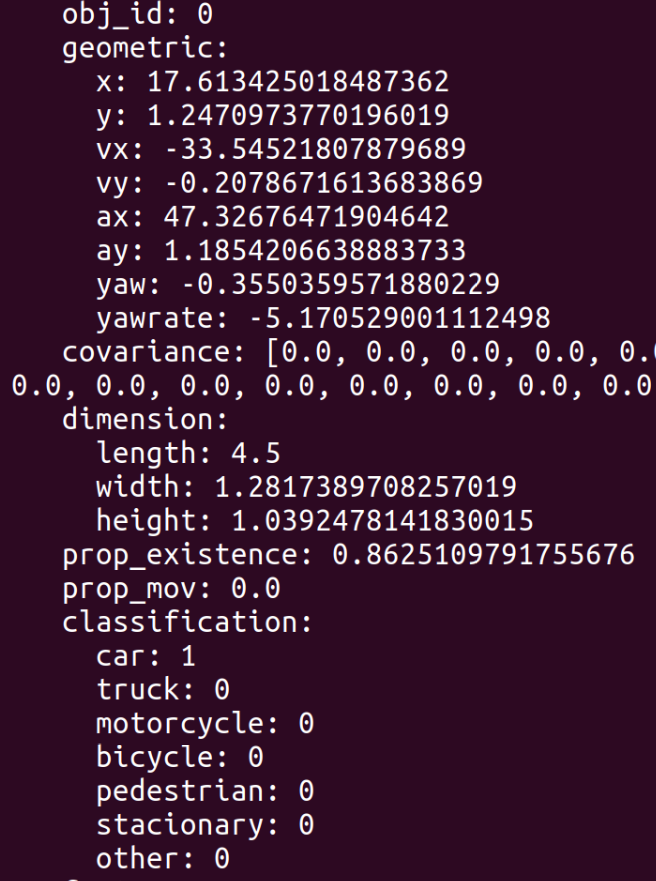
\includegraphics[width=0.3\textwidth]{images/objlist_output.png}
	\caption{Generated Object List}
	\label{fig:ros_outout}
\end{figure}
	\subsection{Visualization of objects lists}

The published topics of \ac{GT} data and Camera-Calculation data are subscribed by \ac{ROS} node \textit{Object\_Visualization}. Each topic contains the ego-vehicle data and the specifically generated objects list. In \ac{RVIZ} the objects are represented by primitive figures with the help of marker messages. Figure \ref{fig:Nodes} shows the used topics and nodes. Rectangles represent topics and ellipses the called nodes. Moreover, tf is a package which controls the coordinate relationship of the ego-vehicle.
\begin{figure*}[thpb]
	\centering
	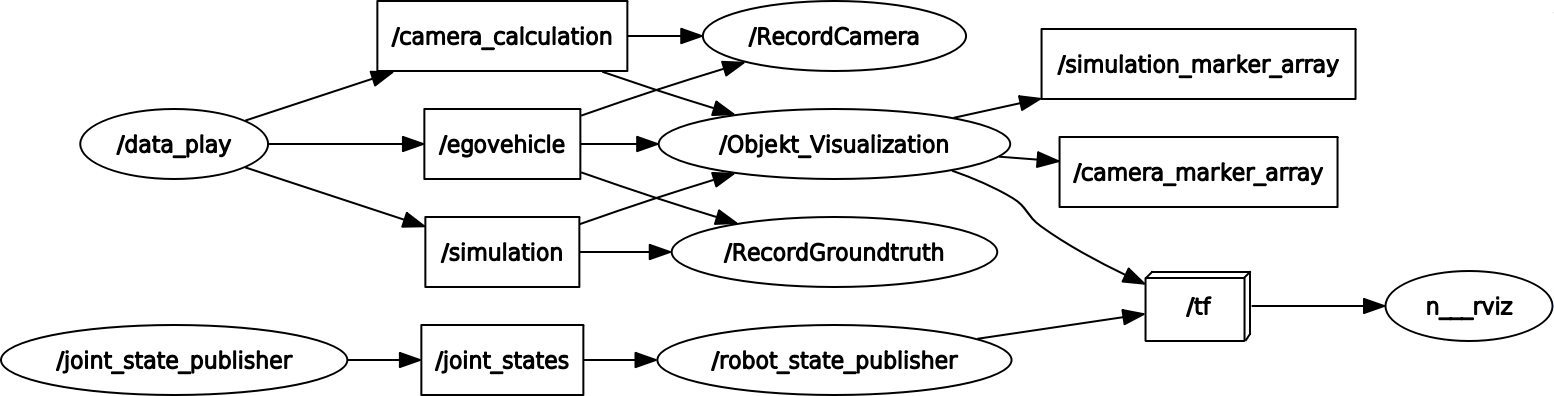
\includegraphics[width=0.85\linewidth]{rosgraph}
	\caption{Nodes (ellipses)/ Topics (rectangles) in \ac{ROS}}
	\label{fig:Nodes}
\end{figure*}
Marker messages are described with specific properties such as position, scale, type, color, orientation. Each object classification is assigned to one specific shape and color so that they can be differentiated in \ac{RVIZ}. The display variants for the possible object classes are shown in \cref{ClassificationAssignment}. 
\begin{table}[h]
	\caption{Classification Assignment}
	\begin{tabularx}{\columnwidth}{XXX}
		\toprule
		Classification & Shape & Color [RGB]\\
		\toprule
		car & cube & [1, 0, 0]\\
		truck & cube & [0, 1, 0]\\
		pedestrian & cylinder & [0, 0, 1]\\
		motorcyle & cube & [1, 0, 1]\\
		bicycle & cylinder & [1, 1, 0]\\
		stacionary & sphere & [0, 1, 1]\\
		other & sphere & [1, 1, 1]\\
		\bottomrule
	\end{tabularx}
	\label{ClassificationAssignment}
\end{table}

In addition, the yaw angle of the objects has to be transformed into a quaternion for the visualization in \ac{RVIZ}. The RGB alpha value of all markers for the calculated camera data is set to 0.5 so that the difference between camera data and GT data is visually recognizable. 
The highest detection probability of an object indicates the classification so that the marker message properties can be set to the corresponding values of \cref{ClassificationAssignment}. Furthermore, each detection position is mirrored on the Y-axis, because the vehicle coordinate system does not match the \ac{RVIZ} coordinate system. Finally, the generated markers are combined into a marker array and published.
The ego-vehicle is described as URDF model according to \cite{URDF}.
Furthermore, the model can be moved and rotated in the \ac{RVIZ} coordinate system by tf messages. 
The published topics of \ac{GT} data, Camera-Calculation data and ego-vehicle data are also saved in a Rosbag file. Each file contains the published ego data and the corresponding objects lists. In the following, these files are used for post-processing.
	\subsection{Evaluation of object lists - Post processing}

After recording object list data streams in Rosbag files there is the possibility to analyse data in different ways by the post processing application offline. The user can either analyse single data streams or compare two different ones. An essential usage would be the comparison of a simulation data stream (Ground-Truth data) to a sensor data stream (camera data). The post processing application provides the opportunity to display several data values within the recorded Rosbag file relating to contained message frames.

\subsubsection{Basic analysis}

Considered to one single Rosbag file specific attribute values of single objects which are selected by their object ID can be displayed. The variety of available attribute types is shown in table 
%\ref{<Object list – attributes table (TP1)>}
. In addition, the number of detected objects can be visualized. 

\subsubsection{Advanced analysis}

Regarding two Rosbag recordings further analysis methods for comparing the streams are provided. In this case a common time base needs to be generated. To avoid errors because of time variation of both recordings following mapping algorithm is executed. Each frame time stamp is handled as time relative to its Rosbag start time in milliseconds. To every frame in the Rosbag file which is provided by sensor data a frame of simulation data is dedicated. The simulation frame to choose is the latest past frame in relative stream time. The principle of frame mapping is shown in figure \ref{fig:frame_mapping}. With this mechanism pairs of frames are generated (sensor frame with corresponding simulation frame).

\begin{figure}[thpb]
	\centering
	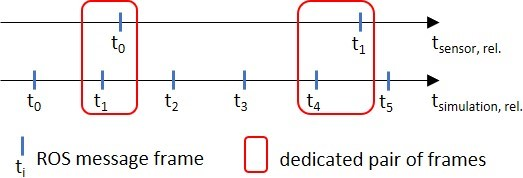
\includegraphics[width=\linewidth]{frame_mapping}
	\caption{Principle of frame mapping algorithm}
	\label{fig:frame_mapping}
\end{figure}

A fundamental use case in analysing the recorded Rosbag files is to evaluate the quality of sensor data. Therefore, it is necessary to operate the mapping of object detection by the sensor in comparison to the simulation data. For this purpose, the algorithm \textbf{Intersection over Union} is applied.

%\include{<Intersection_over_Union (Max H.)>}

!! Put part of Max H. (IoU) here !!

As a result of object mapping it is possible to visualize the number of True Positive (TP), False Positive (FP), False Negative (FN) and mismatch (mm) cases per frame. Further, following quality of service parameter according to \ref{<IEEE paper Fabio Reway>} can be displayed:

\begin{itemize}
	
	\item recall per frame
	\item precision per frame
	\item FPPI per data stream (sensor)
	\item MOTA per data stream (sensor)
	\item MOTP per data stream (sensor)
	
\end{itemize}

Another feature of the post processing application is the analysis of deviations by calculating differences of specific attribute values between two recorded data streams. For that matter only True Positive cases in object mapping are regarded and the concerning object is selected by its object ID in the simulation data record. The difference value results from

$$
difference = value_{simulation} - value_{sensor} \eqno{(???)}
$$

On top of every post processing analysis - except from FPPI, MOTA and MOTP - the mean value and standard deviation of the corresponding value series are calculated.
	
	%%%%%%%%%%%%%%%%%%%%%%%%%%%%%%%%%%%%%%%%%%%%%%%%%%%%%%%%%%%%%%%%%%%%%%%%%%%%%%%%%%
	%%									Results 									%%
	%%%%%%%%%%%%%%%%%%%%%%%%%%%%%%%%%%%%%%%%%%%%%%%%%%%%%%%%%%%%%%%%%%%%%%%%%%%%%%%%%%
	\section{Results}\label{Results}

	Considering the objects lists created by data processing it is noticeable that the camera data is quite different from the \ac{GT} data. Because the simulation is subject to near real-time requirements, a fast processing time is essential. The evaluation and tracking of camera data needs at least 1 second, hence is not fast enough to deliver comparable results. This delay leads to a perceptible offset in the visualization, therefore it is hardly possible to measure the precision of \ac{YOLO} and the calculation.
	Furthermore, minor errors occur with slightly misplaced bounding boxes by \ac{YOLO} and detecting the object precisely within the given bounding box. This influences following values like calculation of the object length and object height.\\
	
	% TODO: in Kapitel RESULTS kopieren
	% TODO: Auswerten
	% Vorausgehende Beschreibung der Situation
	% Wie viele Objekte werden erkannt?
	% Wie viele Objekte werden gematcht?
	% evtl. vergleichende Tabelle bei verschiedenen Threshold-Werten
	% Tabellen mit FPPI, MOTP, MOTA bei versch. Threshold-Werten
	The performance of processed camera data can be evaluated with metrics presented in \cite{Reway} which are realized like introduced in part \ref{sssec:eval}. The metrics are validated by comparing two identical rosbags. This ensures that the implementation of the evaluation functions are correctly. Abbildung Ref shows the distance of an object in x direction from Ground-Truth Data and camera data. Moreover, this figure  makes the time difference between GT and camera data very clearly. The GT stops sending after about nine seconds, because the used sensor suit  can not recognize an object anymore. Certainly, the Camera-Data  sends the comparable object list after another two seconds, so that a correct evaluation can not be carried out. 
	
%	For the given scenario the reached performance is shown in table \ref{tab:res}.
%	
%	\begin{table}[h]
%		\caption{Performance results}
%		\begin{tabularx}{\columnwidth}{XXXX}
%			\toprule
%			\textbf{threshold} & $t=0.5$ & $t=0.6$ & $t=0.7$ \\
%			\toprule
%			Precision & ... & ... & ... \\
%			\midrule
%			Recall & ... & ... & ... \\
%			\midrule		
%			FPPI & ... & ... & ... \\
%			\midrule
%			MOTA & ... & ... & ... \\
%			\midrule
%			MOTP & ... & ... & ... \\
%			\bottomrule
%		\end{tabularx}
%		\label{tab:res}
%	\end{table}
	
	%%%%%%%%%%%%%%%%%%%%%%%%%%%%%%%%%%%%%%%%%%%%%%%%%%%%%%%%%%%%%%%%%%%%%%%%%%%%%%%%%%
	%%									Conclusion									%%
	%%%%%%%%%%%%%%%%%%%%%%%%%%%%%%%%%%%%%%%%%%%%%%%%%%%%%%%%%%%%%%%%%%%%%%%%%%%%%%%%%%
	\section{Conclusions}
	 Nowadays, urban driving simulation software has a major impact on the development process of new autonomous driving functions. Due to the constant further development of the range of functions, the adaptable \ac{API}, \ac{ROS} integration and as well the rapidly growing community, open-source simulators like CARLA offer excellent opportunities for testing and evaluating individual sensor suites and functions. Freely adaptable scenarios and weather conditions offer the developer a lot of flexibility when creating their own test cases.
	 
	 
	 
	 In this specific scenario a real-time object detection system combined with an object tracker are used.
	 As said in \cref{C}, the data processing time is highly dependent on the hardware on which the calculation runs. The delay mentioned in \cref{Results} between the time of recording and visualization leads to outdated results in \ac{RVIZ}. This makes it the most urgent problem to be solved. Further improvements can be achieved with training the \ac{YOLO} algorithm. Synchronizing the published objects lists data by considering the time stamps of the calculated data as well as the \ac{GT} data should also lead to more comparable data. However, this only will be useful if the acquisition time by \ac{YOLO} and the code itself will improve.
	 
	 
%	  to adapt the simulation environment or to synchronize the published frames by considering the time stamps of the calculated data as well as the \ac{GT} data.
	 %Verbesserungen ..... Yolo, Zeit, weigths, frames
	 %Außerem hardware, da Simulation recehnintesiv

	 
	 
	 %Conclusion
	 % wegen 1 Sek Code kann optimiert werden --> 0.3 Sekunden (YOLO) ist aber immer noch zu lange für eine Praxisanwendung
	 % Verbesserung durch 3D-YOLO, YOLO für spezifischen Anwendungsfall antrainieren (nur für relevante Objekte), damit keine Filter mehr notwendig
	 % Frames synchronisieren!!!
	  
	 % Entweder leistungsfähigere Hardware für Echtzeit-Anforderung oder Code-Optimierung
	 % Dadurch signifikante Verbeserung der Rechenzeit möglich
	 
	 
	 
	
	 
	 
	
	 
	
	 
	 
	 
	
	

	%%%%%%%%%%%%%%%%%%%%%%%%%%%%%%%%%%%%%%%%%%%%%%%%%%%%%%%%%%%%%%%%%%%%%%%%%%%%%%%%%%
	%%							Appendix & Acknowledgment							%%
	%%%%%%%%%%%%%%%%%%%%%%%%%%%%%%%%%%%%%%%%%%%%%%%%%%%%%%%%%%%%%%%%%%%%%%%%%%%%%%%%%%
	%\section*{APPENDIX}
	
	Appendixes should appear before the acknowledgment.
	
\section*{ACKNOWLEDGMENT}
	Here comes the acknowledgment
%	The preferred spelling of the word ÒacknowledgmentÓ in America is without an ÒeÓ after the ÒgÓ. Avoid the stilted expression, ÒOne of us (R. B. G.) thanks . . .Ó  Instead, try ÒR. B. G. thanksÓ. Put sponsor acknowledgments in the unnumbered footnote on the first page.
		
	%%%%%%%%%%%%%%%%%%%%%%%%%%%%%%%%%%%%%%%%%%%%%%%%%%%%%%%%%%%%%%%%%%%%%%%%%%%%%%%%
	
%	References are important to the reader; therefore, each citation must be complete and correct. If at all possible, references should be commonly available publications.

	\addtolength{\textheight}{-12cm}    % This command serves to balance the column lengths
										% on the last page of the document manually. It shortens
										% the textheight of the last page by a suitable amount.
										% This command does not take effect until the next page
										% so it should come on the page before the last. Make
										% sure that you do not shorten the textheight too much.

	\bibliographystyle{IEEEtran}{
	\bibliography{Example}}



\end{document}
